% status: 100
% chapter: IaaS

\title{Azure Cosmos DB}


\author{Tolu Agunbiade}
\affiliation{%
  \institution{Indiana University}
  \city{Bloomington} 
  \state{Indiana} 
  \postcode{47408}
}
\email{toagun@iu.edu}

% The default list of authors is too long for headers}
\renewcommand{\shortauthors}{T. Agunbiade}


\begin{abstract}
Azure Cosmos DB is Microsoft's globally distributed, multi-model
database service designed for developers who build mission-critical
applications that require global horizontal scale out
capabilities. Azure Cosmos DB allows customers to elastically scale
across any number of geographical regions while delivering a
financially-backed SLAs for high availability, performance, latency,
and consistency.  This paper will discuss the various features and
capabilities of Azure Cosmos DB and how it solves unique distributed
database challenges.  A basic understanding of distributed database
concept is assumed to understand the content of this paper.
\end{abstract}

\keywords{hid-sp18-501, Microsoft, Storage, Azure, Cosmos DB}


\maketitle

\section{Introduction}
Increasingly, managing data is a critical part of app development and
computing generally. Whether it’s a game, news, travel or fashion app,
it’s always all about the data. For example (cite1) according to
Go-Globe.com~\cite{hid-sp18-501-chameleon}, every 60 seconds, 320 new
accounts and 98,000 tweets are generated on Twitter, about 168,000,000
emails are sent, there are 695,000 status updates, 79,364 wall posts
and 510,040 comments are published on Facebook and so on. These
examples demonstrate the ubiquitous nature of data as well as the need
to manage such a huge volume. Beyond big data management, modern apps
also require databases that is always on, can enable customers to
elastically and globally scale throughput and storage based on demand
and support multiple data models and popular APIs for accessing data.
Azure Cosmos DB is designed to address the challenges described
above. It is a globally distributed database that offers users high
throughput, 99th percentile availability, latency and
consistency. Azure Cosmos DB also supports multi-tenancy and global
distribution. The following sections describe the capabilities of
Azure Cosmos DB.


\section{Features}

\subsection{Global Distribution Architecture}
(cite 2) Azure Cosmos DB is designed so that resources are distributed
along two dimensions: within a given region, all resources are
horizontally partitioned using resource partitions (local
distribution)~\cite{hid-sp18-501-AzureBlog}. Furthermore, each
resource partition is also replicated across geographical regions
(global distribution). Figure~\ref{f:architecture} shows the global
distribution architecture for Cosmos DB.


\begin{figure*}[!ht]
  \centering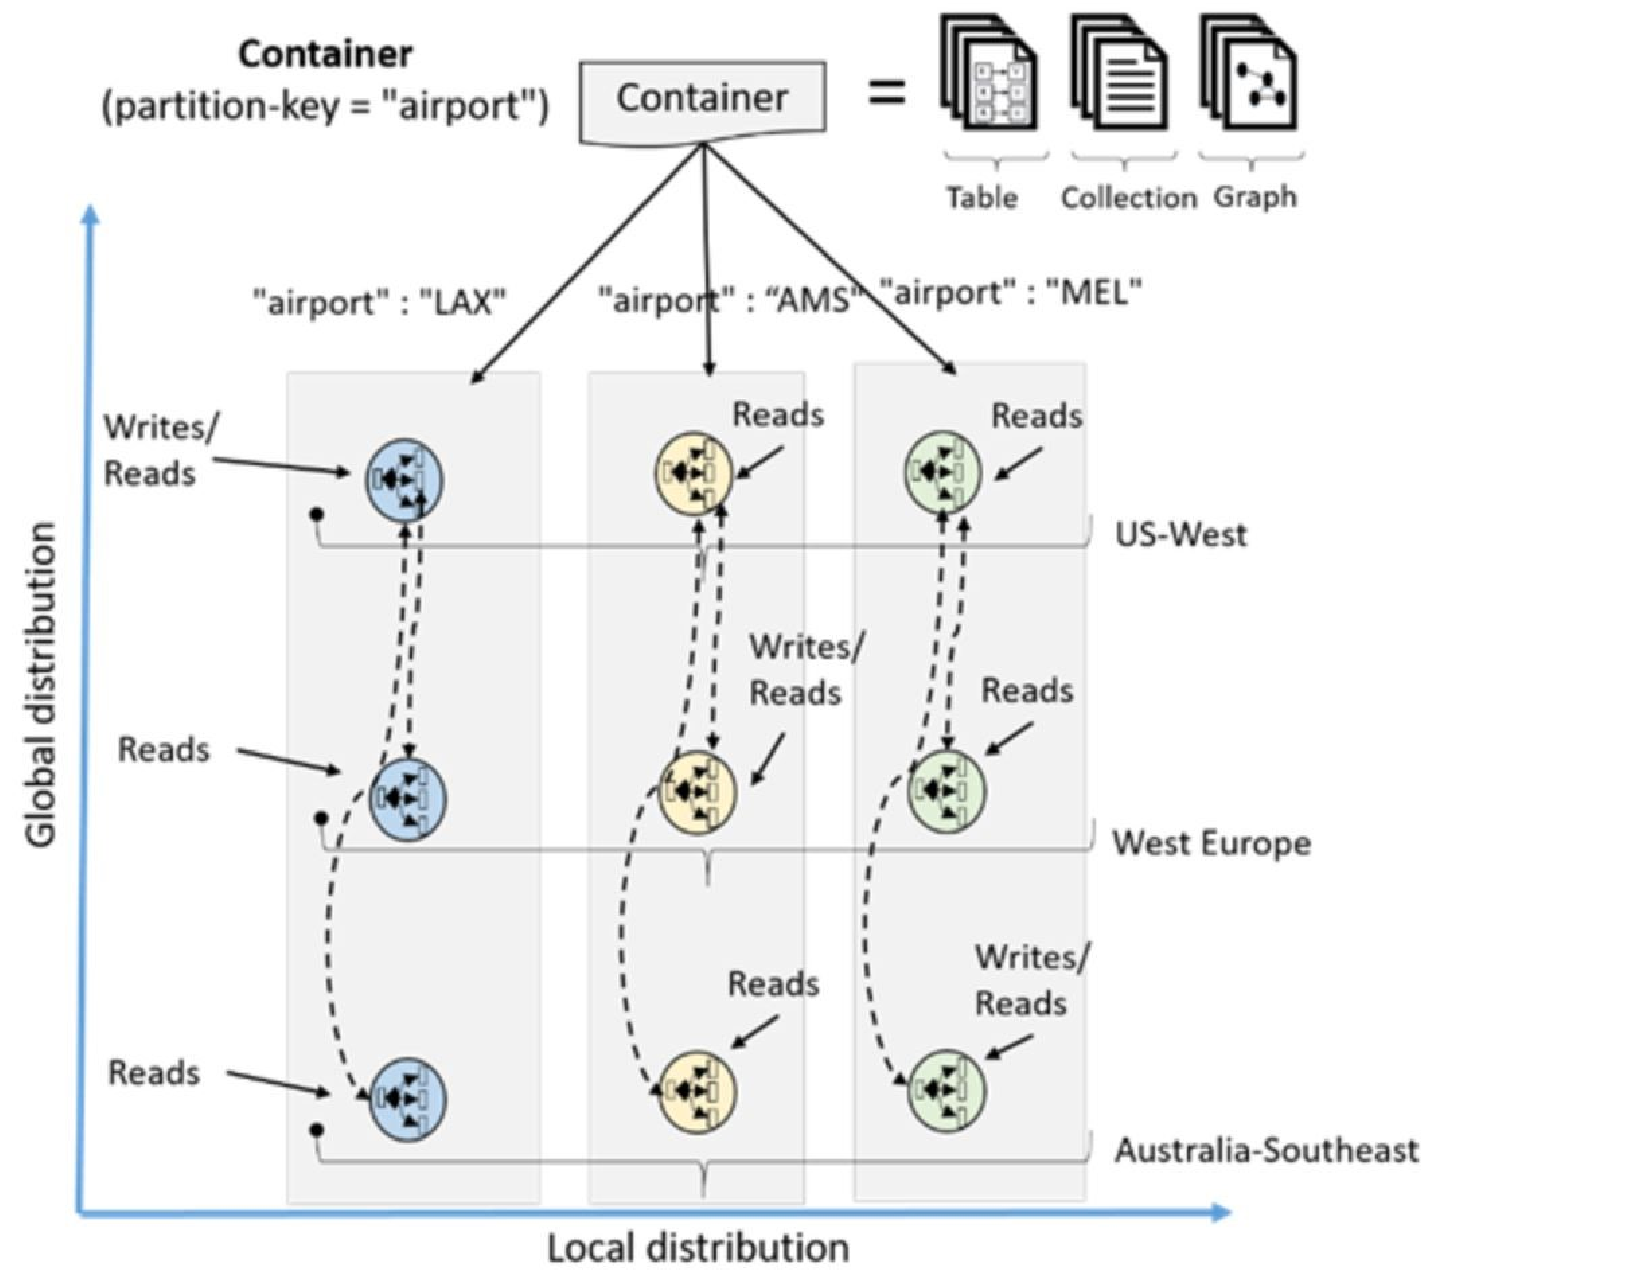
\includegraphics[width=\columnwidth]{images/globe.pdf}
  \caption{Cosmos DB Distribution Architecture~\cite{hid-sp18-501-AzureBlog}}
\label{f:architecture}
\end{figure*}


To scale throughput or storage, Azure Cosmos DB transparently performs
partition management operations across all the regions. Independent of
the scale, distribution, or failures, Azure Cosmos DB continues to
provide a single system image of the globally-distributed
resources. Global distribution of resources in Azure Cosmos DB is
turnkey: at any time with a few clicks or programmatically with a
single API call. Regardless of the amount of data or the number of
regions, Azure Cosmos DB guarantees each newly associated region to
start processing client requests in under an hour at the 99th
percentile. This is done by parallelizing the seeding and copying data
from all the source resource partitions to the newly associated
region. An existing region can also be removed or taken offline.

\subsection{Indexing and Querying}
Azure Cosmos DB’s automatic indexing feature indexes all data
properties. With Azure Cosmos DB, users do not need to decide up front
which elements they're likely to query on. Azure Cosmos DB does not
expect or require any schema or secondary index definitions to index
data at scale. It is truly schema-agnostic. Indexes can be customized
where required to remove unused attributes and elements.  Azure Cosmos
DB also provides rich querying capabilities (SQL, MongoDB, Gremlin
(graph database), Table) with projections, filters, aggregate, sort
and flatten operators, expressions (arithmetic, logical, and various
data transformation). Spatial data types and queries are also
provided.

\subsection{Replication, Consistency and Transactions}
Generally, most distributed databases offer either strong consistency
or eventual consistency. In contrast, Azure Cosmos DB provides a
control of consistency with five well defined consistency levels. A
default account consistency level is configured for write operations;
developers may then ‘weaken’ reads on per request basis. Levels:
Strong, Time Bounded Staleness, Session (Read Your Own Writes),
Consistent Prefix, Eventual.  Azure Cosmos DB allows users to specify
either single partition collections or partitioned collections. Single
partition collections are limited to 10GB/10kRUs. Partitioned
collections on the other hand have no theoretical limit to
scale. Queries may span multiple partitions, but transactions are
always bounded to within a single partition.  Azure Cosmos DB also
support geo-local reads and writes, Elastic scaling throughput,
failover priorities and consistent database schema and index
migration.  Users can dynamically associate “priorities” to the
regions associated with their database account. Priorities are used to
direct the requests to specific regions in the event of regional
failures. In an unlikely event of a regional disaster, Azure Cosmos DB
will automatically failover in the order of priority. In order to test
the end-to-end availability of the application, users can manually
trigger failover (rate limited to two operations within an
hour). Azure Cosmos DB guarantees zero data loss in the case of
customer triggered regional failover and guarantees an upper-bound on
data loss in the event of a system-triggered automatic failover during
a regional disaster. The application does not need to be redeployed
upon regional failover, and the availability SLAs are maintained. For
this, Azure Cosmos DB allows developers to interact with their
resources using either logical (region-agnostic) or physical
(region-specific) endpoints. The former ensures that the application
can transparently be multi-homed in case of failover; the latter
provides fine-grained control to the application to redirect reads and
writes to specific regions. The availability guarantees are agnostic
of the scale (throughput and storage associated with a customer’s
database), number of regions, or geographical distance between regions
associated with a given database.

\subsection{Data Analytics, Full-Text Search and Mobile}
For data analytics, there is direct connectivity from analytics tools
such as Power BI to Azure Cosmos DB. Furthermore, Azure Search and
Azure Cosmos DB offer native integration through the use of
Indexers. The creation and management of data sources (including Azure
Cosmos DB) and indexers that operate against those data sources allows
Azure Cosmos DB content to be indexed and queried from Azure
Search. For mobile app development, Azure Cosmos DB also provides a
native integration with Xamarin (a multi-platform app development
tool) allowing those apps to be able to store data in the cloud.

\subsection{Schema and Data Type Support}
Azure Cosmos DB provides a true schema-agnostic data model while
indexing all data types (documents, graphs, tables). Schema could be
enforced if required using the Javascript trigger capability.  Azure
Cosmos DB entities are stored as JSON. Primitive data type support is
as per JSON (implementation of ARS – atoms, records and
sequences). Spatial types are supported using GeoJSON encoding and
spatial indexing and queries are supported using the WGS-84
co-ordinate system. Both distance and within spatial operators are
provided; collections must be explicitly enabled for spatial data type
indexing.

\subsection{Programmability, Tools and Client SDKs}
Azure Cosmos DB provides rich Javascript based programmability for
SPROC, triggers and UDFs. Javascript provides a mechanism to support
atomic transactional operations and to improve performance by reducing
round-trip calls to the service by shredding and manipulating input
service side.  The Cosmos DB endpoints are standard REST endpoints
with JSON payload. A SQL like query syntax is also provided along with
SDKs for dotNET, Node, Java and Python. Azure Cosmos DB also provides
MongoDB protocol compatibility meaning that many MongoDB drivers and
supported tools will also work.

\subsection{Management and Monitoring}
For Azure Cosmos DB, the Azure portal provides CRUD support with
syntax highlighting and other IDE-like features including Data
Explorer (Graph, Documents, Table). The Microsoft Visual Studio IDE
also provides support for Azure Cosmos DB.  Query execution returns
basic statistics about Resource Units consumed, but there is no
query-plan mechanism to return a detailed query execution plan from
the service.  Cosmos DB has a fully automatic, online backup which is
done approximately every 4 hours and the last 2 backups are stored at
all times. These backups are stored in Azure Blob Storage to guarantee
low latency and efficient upload.


\subsection{Security and Encryption}
Authentication to Azure Cosmos DB is by way of master keys and
delegated resource tokens. Master keys can be retrieved from and reset
via the management portal. Azure Cosmos DB is also integrated with
Azure Active Directory at this time.  Permissions can be granted at
any level of the resource hierarchy; database, collection, document or
attachment; this provides item level permission
granularity. Permissions are either All which grants full CRUD access
or read-only. Execution of procedures requires an All permissions
token on the collection.   Client to service connections must be
secured with SSL. Azure Cosmos DB does not support encryption at
rest. User requiring an audit capability would need to implement this
themselves using triggers.

\subsection{Stack Governance}
Azure Cosmos DB is designed to allow users to elastically scale
throughput based on the application traffic patterns across different
regions to support fluctuating workloads varying both by geography and
time. Operating hundreds of thousands of globally distributed and
diverse workloads cost-effectively requires fine-grained
multi-tenancy, where hundreds of customers share the same machine and
yet thousands share the same cluster. As a resource governed system,
Azure Cosmos DB is a massively distributed queuing system with
cascaded stages of components, each carefully calibrated to deliver
predictable throughput while operating within the allotted budget of
system resources. In order to optimally utilize the system resources
(CPU, memory, disk, and network) available within a given cluster,
every machine in the cluster is capable of dynamically hosting from
10s to 100s of entities. Rate-limiting and back-pressure are plumbed
across the entire stack from the admission control to all I/O
paths. Our database engine is designed to exploit fine-grained
concurrency and to deliver high throughput while operating within
frugal amounts of system resources.  The number of database operations
issued within a unit of time (i.e., throughput) is the fundamental
unit of reservation and consumption of system resources. Users can
perform wide range of database operations against their
data. Depending on the operation type and the size of (the request and
response) payload the operation may consume different amounts of
system resources. Azure Cosmos DB is designed to include an abstract
rate-based currency for throughput called Request Unit or RU which is
available in two denominations based on the time granularity - request
units/sec (RU/s) and request units per minute (RU/m). Users can
therefore elastically scale throughput of a container by
programmatically provisioning RU/s (and/or RU/m) on a
container. Internally, the system manages resource partitions to
deliver the throughput on a given container. Elastically scaling
throughput using horizontally partitioning of resources requires that
each resource partition is capable of delivering the portion of the
overall throughput for a given budget of system resources.

\section{Conclusion}
Modern application development requires database that ensures Global
distribution, elastic horizontal scalability, and multi-model and that
is schema-agnostic. Azure Cosmos DB is designed with these
requirements in mind. As a cloud-born multi-tenant database system,
Azure Cosmos DB’s design interleaves resource governance across its
entire stack. The system is designed from the ground up to offer
global distribution of data, multiple well-defined consistency levels,
ability to elastically scale throughput across geographical regions,
and comprehensive SLAs encompassing throughput, consistency, latency,
and availability to all users and apps.

\begin{acks}

  The author would like to thank Dr.~Gregor~von~Laszewski for his
  support and suggestions in writing this paper.

\end{acks}

\bibliographystyle{ACM-Reference-Format}
\bibliography{report} 

